\chapter{Introduction}
\label{c:intro}

% rise and prominence of cloud storage
\section{Rise and Prominence of Cloud Storage}
\label{s:riseandprominenceofcloudstorage}
Over the past few years, cloud storage has experienced a metamorphosis from a trendy term to a mature technology and successful business. Due to its high reliability, low cost and minimum management overhead, more and more individual users and enterprises have chosen cloud storage as their major storage solution. According to a recent survey from Enterprise Storage Forum\cite{storagetrends2018}, 68\% of the surveyed enterprises includes cloud in their current storage infrastructure and 35\% of them store their company's primary storage data on cloud storage services. Clearly, high cost of storage hardware has lead businesses to outsource the headaches of in-house storage, and cloud storage turns out to be the best alternative.

% concerns of single cloud solution
\section{Concerns of Single Cloud Solution}
\label{s:concernsofsinglecloudsolution}
While cloud has rapidly become the dominant adoption among all kind of storage choices, another aspect of concerns arises. According to a recent market survey done by DataCore\cite{datacore2017survey}, security (57\%), sensitive data (56\%) and regulatory requirements (41\%) were the 3 major concerns that blocks enterprises from migrating to a public cloud. With data outsourced to a third-party cloud provider, privacy settings are beyond the control of the enterprise. In this situation, sensitive data such as banking information or patient's medical records are exposed to the risks of been viewed or mishandled by malicious insiders in the single cloud. In addition, the "single cloud" solution also suffers from some potential risks such as service availability failure or vendor lock-in problem. For example, table \ref{table:cloudstoragecost} shows the major pricing schema of 3 popular cloud storage providers. Besides the monthly per-GB storage fee, consumers also need to pay an non-negligible fee for their per-GB download traffic. As a consequence, with a large amount of data stored on a single cloud, consumers become dependent (i.e. "locked-in") on this vendor's services and are unable to switch to a different vendor - due to the high switching costs.

\begin{table}[!b]
\centering
  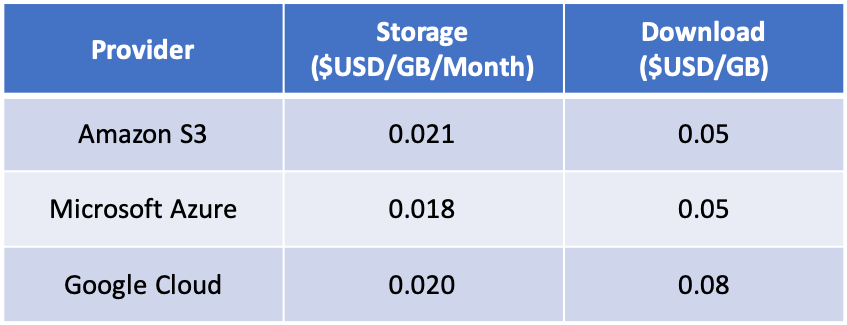
\includegraphics[width=13cm]{tables/table_cloud_storage_cost.png}
  \caption{Major pricing scheme of 3 popular cloud storage providers}
  \label{table:cloudstoragecost}
\end{table}

% FileFarm overview
\section{FileFarm Overview}
\label{s:filefarmoverview}
This thesis focuses on resolving the problems caused by dependence on a single storage provider. To be specific, we propose FileFarm, a cloud-of-clouds storage solution that leverages reliability of public cloud storage services while keeping needs from following aspects:

\begin{enumerate}
    \item Preservation of data security and privacy
    \item No reliance on any single cloud
    \item On-demand flexibility of switching between clouds
    \item Cost efficiency
\end{enumerate}

In FileFarm, storage nodes named "\textit{farmers}" coordinate with each other to constitute a peer-to-peer storage network, in a sense that service availability has no dependence on any single farmer. Thus, there is no single-point-of-failure in the FileFarm storage network. With respect to the working flow, each farmer in FileFarm is linked with exactly 1 storage provider (either a public cloud or a private data server) and runs an independent server that provides storage services in terms of GET, PUT, DELETE APIs. To access FileFarm, an authenticated client establishes a stateless connection with any 1 farmer. Since the services provided by farmers are identical, a client can upload a data chunk to FileFarm through one farmer and download it later through another. FileFarm takes care of redundancy automatically, with redundant copies of data distributed over the network. When a farmer encounters service failure, an additional copy of each data chunk it stored will be stored by another farmer automatically. In case of a new farmer joining the network, storage load on each farmer will be balanced automatically.
